\chapter{Методология решения задач CAPTCHA}

\section{Общие подходы к автоматизированному решению CAPTCHA}

Для автоматизации решения CAPTCHA могут применяться различные методы и подходы, 
которые зависят от конкретной реализации CAPTCHA. В рамках данной работы можно 
выделить следующие методы:
\begin{enumerate}
    \item реализация CAPTCHA в аудиоформате:
    \begin{enumerate}
        \item шумоподавление и фильтрация;
        \item распознавание речи;
        \item преобразование речи в текст.
    \end{enumerate}
    \item реализация CAPTCHA в текстовом формате:
    \begin{enumerate}
        \item бинаризация изображения и фильтрация фона;
        \item сегментация символов;
        \item классификация символов;
        \item распознавание последовательности символов;
        \item аугментация данных;
        \item генерация синтетических датасетов.
    \end{enumerate}
    \item реализация CAPTCHA в графическом формате:
    \begin{enumerate}
        \item нормализация и ручная разметка изображений;
        \item детекция объектов;
        \item сегментация объектов;
        \item классификация фрагментов изображения;
        \item поиск и сопоставление с шаблоном. 
    \end{enumerate}
    \item общие подходы для большинства реализаций:
    \begin{enumerate}
        \item анализ структуры HTML-документа на стороне клиента;
        \item автоматизация кликов и действий на web-странице.
    \end{enumerate}
\end{enumerate}

Для каждого формата одним из основополагающих этапов является этап 
предобработки исходного файла. Для аудиозаписей, которые используются в Audio 
CAPTCHA требуется применить шумоподавление и фильтрацию.

Шумоподавление (шумопонижение) -- процесс устранения или уменьшения нежелательных 
шумов из аудиосигнала с целью повышения его качества или уменьшения уровня ошибок 
при передаче и хранении данных. Методы шумоподавления могут быть реализованы как 
аппаратно, так и программно, и направлены на увеличение отношения сигнал/шум.(https://fastercapital.com/ru/content/%D0%9A%D0%BE%D0%BC%D0%BF%D1%8C%D1%8E%D1%82%D0%B5%D1%80%D0%BD%D0%B0%D1%8F-%D0%BE%D0%B1%D1%80%D0%B0%D0%B1%D0%BE%D1%82%D0%BA%D0%B0-%D0%B7%D0%B2%D1%83%D0%BA%D0%B0--%D0%BA%D0%B0%D0%BA-%D0%BE%D0%B1%D1%80%D0%B0%D0%B1%D0%B0%D1%82%D1%8B%D0%B2%D0%B0%D1%82%D1%8C-%D0%B8-%D1%83%D0%BB%D1%83%D1%87%D1%88%D0%B0%D1%82%D1%8C-%D0%B7%D0%B2%D1%83%D0%BA-%D1%81-%D0%BF%D0%BE%D0%BC%D0%BE%D1%89%D1%8C%D1%8E-%D0%BA%D0%BE%D0%BC%D0%BF%D1%8C%D1%8E%D1%82%D0%B5%D1%80%D0%BE%D0%B2.html)

Фильтрация -- процесс удаления или ослабления определенных частотных составляющих 
аудиосигнала при сохранении других. Фильтрацию можно использовать для удаления 
шума, частотный спектр которого отличается от желаемого сигнала.

Фильтрация играет важную роль в улучшении качества звучания аудиофайлов, 
эффективном подавлении шумов и помех, а также в создании специальных звуковых 
эффектов.

Для CAPTCHA в текстовом формате в качестве предобработки используется бинаризация 
и фильтрация фоновых шумов для упрощения следующих этапов обработки.

Бинаризация -- процесс преобразования цветного или полутонового изображения в 
двухцветное (черно-белое), где каждый пиксель принимает одно из двух возможных 
значений: 0 (черный) или 1 (белый). Основным параметром бинаризации является 
пороговое значение, с которым сравнивается яркость каждого пикселя. Существуют 
различные методы бинаризации, включая глобальные и локальные подходы.(https://cyberleninka.ru/article/n/issledovanie-metodov-binarizatsii-izobrazheniy/viewer)

Бинаризация широко используется в задачах распознавания текста, где упрощение 
изображения до двух цветов облегчает выделение символов и их последующее 
распознавание.

Фильтрация фонового шума -- процесс удаления или уменьшения нежелательных шумов, 
которые могут мешать анализу или распознаванию содержимого изображения. Шумы 
могут возникать из-за различных факторов, таких как условия съемки, качество 
оборудования или передача данных. В частности, для CAPTCHA фоновые шумы 
генерируются намеренно.

Существует большое количество методов фильтрации шума, включая:
\begin{enumerate}
    \item Гауссов фильтр: используется для размытия изображения с целью удаления 
    высокочастотного шума;
    \item медианный фильтр: заменяет значение каждого пикселя на медиану значений 
    в его окрестности, эффективно устраняя импульсные шумы;(МЕТОДИКА УСТРАНЕНИЯ ШУМА НА ОКТ-ИЗОБРАЖЕНИЯХ)
    \item частотная фильтрация: применяется в частотной области для удаления 
    определенных частотных компонентов, связанных с шумом.(https://www.xn----8sbempclcwd3bmt.xn--p1ai/article/16686)
\end{enumerate}

Эффективная фильтрация фонового шума особенно важна при обработке изображений с 
текстом, так как наличие шума может затруднить или сделать невозможным корректное 
распознавание символов.

Для облегчения работы модели в дальнейшем, для графических CAPTCHA в качестве 
предобработки используется нормализация и ручная разметка изображений датасета.

Нормализация -- процесс приведения изображений к единому стандарту по 
определенным характеристикам, таким как размер, яркость, контрастность или 
геометрические параметры. Целью нормализации является обеспечение однородности 
входных данных для последующей обработки или анализа.(Gonzalez, R. C., \& Woods, R. E. (2018). Digital Image Processing (4th Edition). Pearson)

Разметка изображений -- процесс аннотирования изображений с целью идентификации 
и классификации объектов или областей интереса на изображении. Разметка является 
ключевым этапом в подготовке данных для обучения моделей компьютерного зрения и 
машинного обучения.

Разметка изображений обеспечивает модели данными, необходимыми для обучения 
точному распознаванию и интерпретации визуальной информации. Размеченные 
фотографии используются в различных задачах, от обнаружения объектов до 
автоматической обработки изображений.(https://annotate.ru/blog/semanticheskaya\_razmetka\_dlya\_mashinnogo\_obucheniya)

Дальнейшие подходы и методы связаны непосредственно с поиском решения задания 
CAPTCHA и также специфичны для каждой реализации CAPTCHA.

Распознавание речи -- технология преобразования устной речи в текстовую форму. 
Современные системы ASR (Automatic Speech Recognition) используют глубокие 
нейронные сети для обработки аудиосигналов и преобразования их в текст.(https://www.assemblyai.com/blog/what-is-asr)

Преобразование речи в текст -- процесс транскрибирования устной речи в письменную 
форму. Этот процесс включает в себя анализ аудиосигнала, выделение речевых 
признаков и преобразование их в текст.(https://h2o.ai/wiki/speech-to-text/)

Задача сегментации представляет из себя процесс разделения изображения на 
дискретные группы пикселей для обнаружения важных участков изображения или 
объектов. В задачах компьютерного зрения, таких как распознавание текста на 
изображениях, сегментация помогает выделить отдельные символы или слова для 
последующей обработки.(https://www.ibm.com/think/topics/image-segmentation)

Задача классификации представляет собой процесс присвоения входным данным одной 
из предопределенных категорий. В контексте обработки изображений, классификация 
может использоваться для определения наличия текста на изображении, для 
распознавания символов или различных объектов.(https://www.sciencedirect.com/topics/engineering/image-classification)

Распознавание последовательности символов -- это задача извлечения и 
интерпретации последовательности символов из входных данных, таких как 
изображение или аудиосигнал. В системах OCR (оптического распознавания символов) 
это включает в себя определение порядка символов и их преобразование в текст.($https://aws.amazon.com/what-is/ocr/?nc1=h_ls$)

Аугментация данных -- метод увеличения объема обучающего набора данных путем 
применения различных трансформаций к существующим данным. В задачах обработки 
изображений это может включать повороты, масштабирование, изменение яркости и 
контрастности.(https://www.ibm.com/think/topics/data-augmentation)

Генерация синтетических датасетов -- процесс создания искусственных данных для 
обучения моделей машинного обучения. Это особенно полезно, когда реальные данные 
ограничены или трудно доступны.(https://www.nvidia.com/en-us/glossary/synthetic-data-generation/)

Детекция объектов -- задача определения и локализации объектов на изображении. В 
системах CAPTCHA это может использоваться для идентификации определенных 
элементов, таких как дорожные знаки или транспортные средства.(https://www.ibm.com/think/topics/object-detection)

Поиск и сопоставление с шаблоном -- метод обработки изображений, используемый 
для поиска частей входного изображения (большого изображения или целевого 
изображения), которые соответствуют шаблонному изображению (эталонному 
изображению или меньшему изображению). Сопоставление шаблонов обычно 
используется для задач обнаружения объектов, распознавания изображений и 
распознавания образов.(https://blog.roboflow.com/template-matching/)

Также, задача автоматизации решения CAPTCHA была бы нерешаема без 
непосредственного взаимодействия с браузером без участия пользователя, для чего 
применяются описанные ниже подходы.

Анализ структуры HTML-страницы -- процесс разбора и интерпретации HTML-кода 
web-страницы для извлечения информации или автоматизации взаимодействия с 
элементами страницы.(https://www.geeksforgeeks.org/html-parsing-and-processing/)

Автоматизация действий пользователя -- это использование программных средств для 
имитации действий пользователя, таких как клики мышью, ввод текста или навигация 
по интерфейсу. Это может применяться для автоматического прохождения CAPTCHA или 
тестирования пользовательских интерфейсов.(https://www.testresults.io/definitions/automated-user-interaction)

\section{Архитектуры нейронных сетей для различных форматов CAPTCHA}

В данной работе рассмотрены три наиболее популярные и частовстречающиеся 
реализации CAPTCHA, которые применяются для защиты web-ресурсов: аудио CAPTCHA, 
текстовые CAPTCHA и графические CAPTCHA (CAPTCHA с изображениями). Для каждой 
реализации необходим свой подход к решению, разный набор инструментов и библиотек.

Далее для каждой из реализаций будцт рассмотрены различные архитектуры нейронных 
сетей, которые могут быть использованы для автоматизации решения CAPTCHA.

\textbf{Архитектуры нейронных сетей для текстовых CAPTCHA}

Для задачи решения текстовых CAPTCHA могут быть использованы различные модели 
нейронных сетей, которые поддерживают обработку последовательностей различной 
длины. Среди таких архитектур и инструментов можно выделить следующие:
\begin{enumerate}
    \item оптическое распознавание символов (Tesseract OCR);
    \item cверточные рекурентные нейронные сети с функцией потерь Connectionist 
    Temporal Classification (CRNN + CTC);
    \item архитектура последовательного обучения (Sequence-to-Sequence).
\end{enumerate}

Tesseract OCR -- это свободный движок оптического распознавания текста, 
изначально разработанный в Hewlett-Packard в 1985–1995 годах и в дальнейшем 
выпущенный как open-source-проект Google в 2005 году. В настоящее время он 
поддерживается и активно развивается сообществом под эгидой Google. С версии 4.0 
Tesseract использует глубокую нейросетевую архитектуру, что значительно улучшило 
его производительность на задачах распознавания сложных текстов и документов.(An Overview of the Tesseract OCR Engine, Adrian Rosebrock. OCR with OpenCV, Tesseract, and Python. PyImageSearch.)

Основные этапы обработки текста в Tesseract:(Adrian Rosebrock. OCR with OpenCV, Tesseract, and Python. PyImageSearch.)
\begin{enumerate}
    \item предобработка изображения: включает бинаризацию, удаление шумов, 
    коррекцию наклона и выравнивание; эти шаги направлены на улучшение качества 
    входного изображения для более точного распознавания;
    \item разметка структуры документа: изображение разбивается на блоки, строки 
    и отдельные слова; сначала происходит анализ макета документа, включая 
    идентификацию текста, таблиц, изображений и других структур;
    \item распознавание текста: начиная с версии 4.0, Tesseract использует LSTM 
    (Long Short-Term Memory) -- разновидность рекуррентных нейросетей, 
    позволяющую учитывать контекст в последовательности символов; распознавание 
    не требует предварительной сегментации символов -- вместо этого используется 
    подход Connectionist Temporal Classification (CTC), обеспечивающий 
    сопоставление входной последовательности признаков с выходной строкой текста;
    \item постобработка: включает коррекцию ошибок с помощью встроенных языковых 
    моделей, фильтрацию недопустимых символов и оптимизацию финального вывода 
    текста.
\end{enumerate}

Нейросетевой движок в Tesseract 4.0 построен следующим образом:(An Overview of the Tesseract OCR Engine)
\begin{enumerate}
    \item входное изображение пропускается через сверточный слой для извлечения 
    признаков;
    \item далее признаки передаются в двунаправленные LSTM-ячейки, способные 
    учитывать как предыдущий, так и последующий контексты;
    \item выход LSTM обрабатывается функцией CTC, которая выравнивает вероятности 
    символов по времени и строит финальную строку текста.
\end{enumerate}

Архитектура движка Tesseract на примере обработки входной последовательности 
приведена на рис.~\ref{fig:tesseract}.

\begin{figure}[H]
    \centering
    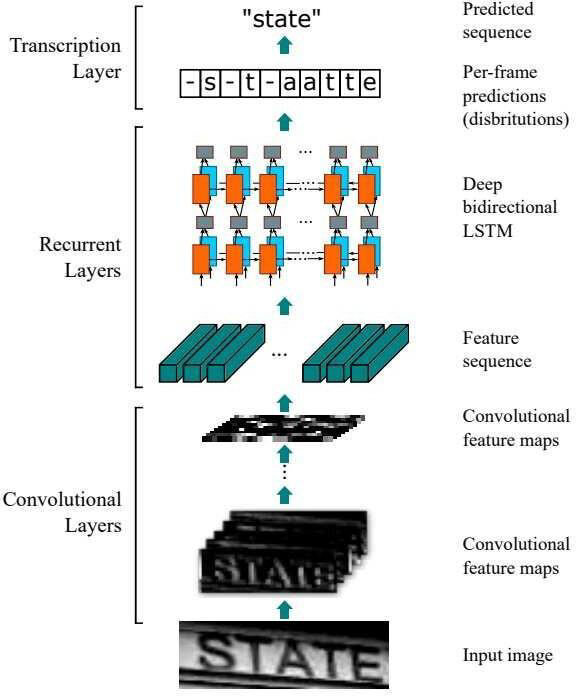
\includegraphics[width=0.75\textwidth]{
        imgs/theory/TesseractOCR.png
    }
    \caption{Архитектура нейросетевого движка Tesseract OCR.}
    \label{fig:tesseract}
\end{figure}
\vspace{-0.85cm}

Этот подход особенно устойчив к искажениям и перемещениям текста, поскольку 
модель обучается <<видеть>> всю строку целиком, а не по символам.

Преимущества Tesseract:(Adrian Rosebrock. OCR with OpenCV, Tesseract, and Python. PyImageSearch.)
\begin{enumerate}
    \item гибкость: поддержка множества языков, включая написание справа-налево, 
    китайский, японский и арабский;
    \item обучаемость: пользователь может дообучать модель на своих собственных 
    данных;
    \item интеграция: легко используется совместно с библиотеками обработки 
    изображений, такими как OpenCV.
\end{enumerate}

Архитектура CRNN (Convolutional Recurrent Neural Network) с CTC (Connectionist 
Temporal Classification) -- это специализированный подход к распознаванию 
последовательностей на входах переменной длины. Он широко применяется в OCR, 
распознавании речи и жестов, где отсутствует строгое выравнивание между входами 
и метками.(Ian Goodfellow, Yoshua Bengio, Aaron Courville. Deep Learning)

Данный подход объединяет сверточные нейронные сети (для извлечения признаков), 
рекуррентные нейронные сети (для моделирования зависимости во 
времени/пространстве) и CTC (для сопоставления выходной последовательности с 
целевым результатом без предварительной сегментации).

Первая составляющая архитектуры -- сверточная нейронная сеть (CNN), задача 
которой -- извлечь дискретные признаки из исходного изображения (например, строки 
текста, номера или CAPTCHA).

Архитектура сверточных нейронных сетей состоит из комбинации слоев:
\begin{enumerate}
    \item сверточные слои, извлекают локальные пространственные шаблоны 
    (например, края, формы);
    \item пуллинговые слои, которые уменьшают размерность и повышают 
    инвариантность;
    \item выходной слой, который представляет собой матрицу признаков, часто 
    сжатую по вертикали, но сохраняющую пространственную структуру по ширине, 
    что формирует последовательность признаков, где каждый вектор соответствует 
    <<временной метке>> (например, потенциальному символу).
\end{enumerate}

После получения последовательности признаков из CNN, она поступает на вход 
рекуррентной нейронной сети для анализа временной структуры последовательности 
признаков. Наиболее часто используется двунаправленная LSTM, поскольку она 
обрабатывает последовательность слева направо и справа налево, позволяя учитывать 
как предшествующий, так и последующий контекст, что особенно важно при наличии 
похожих символов и искажений.(Ian Goodfellow, Yoshua Bengio, Aaron Courville. Deep Learning)

Результатом является последовательность выходных векторов, каждый из которых 
соответствует одному <<временному шагу>> -- потенциальному символу.

Выходы из рекуррентной части подаются на полносвязный слой (или линейную 
проекцию), где каждый вектор переводится в вектор вероятностей по алфавиту 
(включая специальный пустой символ, обозначающий отсутствие выхода).

Затем применяется Connectionist Temporal Classification -- специализированная 
функция потерь, предназначенная для задач, где отсутствует выравнивание между 
входной и выходной последовательностью.(Connectionist Temporal Classification: Labelling Unsegmented
Sequence Data with Recurrent Neural Networks)

Connectionist Temporal Classification обладает следующими особенностями:
\begin{enumerate}
    \item не требует сегментации или аннотированных позиций символов;
    \item поддерживает множество путей к одному выходу;
    \item вводит символ <<blank>> для обозначения промежутков или 
    неопределенности;
    \item обеспечивает обучение <<end-to-end>> на уровне целых строк текста.
\end{enumerate}

Архитектура Sequence-to-Sequence (Seq2Seq) представляет собой класс нейронных 
сетей, предназначенных для преобразования одной последовательности элементов в 
другую, при этом длины входной и выходной последовательностей могут различаться. 
Первоначально эта архитектура была предложена для задач машинного перевода 
(https://arxiv.org/abs/1409.3215), однако в последующем она нашла широкое применение и в 
других областях, таких как распознавание речи, автоматическая транслитерация, 
генерация текстов и, в частности, распознавание текстовых CAPTCHA.

Основу Seq2Seq составляет двухкомпонентная архитектура: энкодер и декодер. 
Энкодер последовательно обрабатывает входные данные (например, текст или объекты, 
извлеченные из изображения с помощью сверточной сети) и кодирует их в вектор 
фиксированной длины -- так называемый вектор контекста. Декодер, в свою очередь, 
получает этот вектор и генерирует выходную последовательность, по одному элементу 
за шаг, используя скрытое состояние и ранее сгенерированные элементы.

Классическая реализация Seq2Seq использует рекуррентные нейронные сети (RNN), 
включая их модификации -- LSTM и GRU. В энкодере последовательность входных 
векторов обрабатывается пошагово, и финальное скрытое состояние используется как 
компактное представление всей последовательности. Это состояние затем передается 
в декодер, который генерирует выход, начиная с начального маркера.

Одной из ключевых проблем базовой Seq2Seq-модели является невозможность 
эффективно работать с длинными входными последовательностями, поскольку 
информация вектора контекста может быть потеряна. Для преодоления этого 
ограничения была предложена модификация с использованием механизма внимания, 
позволяющего декодеру на каждом шаге фокусироваться на различных частях входной 
последовательности.(https://arxiv.org/abs/1508.04025).

\textbf{Архитектуры нейронных сетей для графических CAPTCHA}

При решении графических CAPTCHA важными являются возможности модели по детекции
и сегментации объектов, поскольку данные CAPTCHA могут требовать как обычного 
поиска объекта, так и выбора клеток, в которых содержится объект. Для решения 
данных задач могут применяться следующие инструменты и архитектуры нейронных 
сетей:
\begin{enumerate}
    \item одноэтапная модель для детекции объектов (YOLO, You Only Look Once);
    \item модель детекции, основанная на архитектуре трансформера (DETR, 
    DEtection TRansformer);
    \item модель сверточной нейронной сети для двухэтапного обнаружения объектов 
    (Faster R-CNN).
\end{enumerate}

YOLO (You Only Look Once) -- семейство нейросетевых моделей, разработанных для 
реализации задачи детекции объектов в изображениях в реальном времени. В отличие 
от традиционных методов, которые разделяют задачу на два этапа (предсказание 
регионов и их классификация), YOLO выполняет эти задачи одновременно в рамках 
единой сверточной нейросети. Первая версия YOLO была представлена Джозефом 
Редмоном и его коллегами в 2016 году, с тех пор были разработаны многочисленные 
улучшенные версии (последняя версия на данный момент YOLOv11), каждая из которых 
повышала точность и скорость работы.

YOLO разделяет входное изображение на сетку $S \times S$, для каждой ячейки сеть 
предсказывает B ограничивающих рамок, а также вероятности принадлежности к 
каждому из классов. Каждое предсказание содержит следующие параметры:
\begin{enumerate}
    \item координаты ограничивающей рамки (центр x, y, ширина w, высота h);
    \item уверенность модели в том, что в рамке находится объект;
    \item вероятности классов (условные вероятности при наличии объекта).
\end{enumerate}

Выход модели представляет собой тензор с размерностью $S \times S \times (B * 5 + 
C)$, где $C$ -- количество классов.

YOLO использует <<end-to-end>> обучение, что позволяет быстро и эффективно 
предсказывать объекты и их классы за один проход изображения через сеть. Это 
особенно важно при применении в задачах CAPTCHA, где требуется обрабатывать 
большое количество мелких изображений в режиме реального времени.

YOLOv11 представляет собой значительный шаг вперед в развитии моделей детекции 
объектов реального времени. Она сочетает в себе высокую точность, эффективность и 
универсальность, что делает ее применимой в различных задачах компьютерного 
зрения, включая распознавание объектов на изображениях CAPTCHA.(https://arxiv.org/abs/1506.02640)

Основные компоненты архитектуры YOLOv11:(https://arxiv.org/abs/2410.17725)
\begin{enumerate}
    \item основная сеть: YOLOv11 использует улучшенный каркас для извлечения 
    признаков, основанный на блоках C3K2 (Cross Stage Partial) с ядром 
    $2\times2$, эти блоки обеспечивают эффективное извлечение признаков при 
    меньших вычислительных затратах, сохраняя при этом способность модели 
    захватывать важные особенности изображения;
    \item связующий модуль: модель внедряет модуль SPPF (Spatial Pyramid 
    Pooling -- Fast), который позволяет эффективно обрабатывать объекты различных 
    масштабов, улучшая способность модели к детекции как крупных, так и мелких 
    объектов;
    \item механизмы внимания: YOLOv11 интегрирует блок C2PSA (Convolutional block 
    with Parallel Spatial Attention), который усиливает способность модели 
    фокусироваться на релевантных частях изображения, улучшая точность детекции, 
    особенно в сложных сценах;
    \item выходной слой: выходной слой модели оптимизирован для быстрого и точного 
    предсказания ограничивающих рамок и классов объектов, обеспечивая 
    высокую производительность в реальном времени.
\end{enumerate}

Модель YOLOv11 обладает следующими преимуществами:
\begin{enumerate}
    \item высокая точность: благодаря улучшенному извлечению признаков и 
    механизмам внимания YOLOv11 демонстрирует высокие показатели точности в 
    задачах детекции объектов;
    \item эффективность: оптимизированная архитектура обеспечивает быстрое 
    выполнение модели, что особенно важно для приложений, требующих обработки в 
    реальном времени;
    \item универсальность: модель поддерживает различные задачи компьютерного 
    зрения, включая детекцию объектов, сегментацию, классификацию и определение 
    позы, что делает ее применимой в широком спектре приложений.
\end{enumerate}

Также, примером современной архитектуры для задачи обнаружения объектов является 
DETR (DEtection TRansformer) -- модель, предложенная исследователями из Facebook 
AI Research в 2020 году (https://arxiv.org/abs/2005.12872). В отличие от 
традиционных сверточных решений, DETR применяет архитектуру трансформера, ранее 
широко использовавшуюся в области обработки естественного языка, для анализа 
визуальных данных. Основной особенностью DETR является переосмысление задачи 
детекции как задачи сопоставления предсказаний с реальными объектами на 
изображении в постановке <<многие ко многим>>.

Архитектура DETR состоит из трех основных компонентов: извлекающей признаковую 
информацию сверточной нейронной сети, архитектуры трансформера (включающей 
энкодер и декодер), а также выходной регрессионно-классификационной части.(https://arxiv.org/abs/2005.12872)

На начальном этапе используется сверточная нейронная сеть, такая как ResNet-50 
или ResNet-101, предназначенная для извлечения признаков изображения. На выходе 
формируется тензор размерности $C \times X \times W$, где $C$ -- число каналов, 
$H$ и $W$ -- пространственные размеры. Этот тензор преобразуется в 
последовательность векторов, которая поступает на вход трансформеру. К каждому 
вектору добавляется позиционная информация, необходимая для сохранения 
пространственной структуры изображения.

Следующим этапом является применение трансформера, включающего энкодер и декодер:
\begin{enumerate}
    \item энкодер принимает последовательность признаков и обрабатывает их с 
    помощью многоголового механизма самовнимания (multi-head self-attention), 
    формируя глобальное представление изображения;
    \item декодер работает с фиксированным набором обучаемых векторов, называемых 
    объектными запросами, каждый из которых предназначен для предсказания одного 
    потенциального объекта, декодер на каждом шаге взаимодействует с выходами 
    энкодера, формируя выходные векторы, соответствующие найденным объектам.
\end{enumerate}

Каждый из выходных векторов декодера передается в многослойный перцептрон, 
предсказывающий класс объекта и координаты ограничивающего прямоугольника. 
Сопоставление между предсказанными и реальными объектами выполняется с 
использованием венгерского алгоритма, что позволяет обучать модель в режиме 
<<end-to-end>> без применения процедур постобработки, таких как подавление 
немаксимумов.

Модель DETR обладает рядом преимуществ по сравнению с традиционными подходами:
\begin{enumerate}
    \item архитектура позволяет отказаться от использования якорей и 
    эвристических алгоритмов;
    \item глобальное внимание трансформера способствует лучшему захвату 
    контекста;
    \item прямое сопоставление предсказаний с объектами упрощает процедуру 
    обучения;
    \item обучение происходит в парадигме <<end-to-end>>.
\end{enumerate}

При этом, оригинальная версия DETR характеризуется сравнительно медленной 
сходимостью, особенно при обучении на малых объемах данных, поэтому с момента 
появления оригинальной версии модели было предложено несколько улучшений, 
направленных на повышение скорости сходимости и качества предсказаний:
\begin{enumerate}
    \item Deformable DETR -- введение деформируемого внимания, ограничивающего 
    область восприятия и позволяющего ускорить обучение;(https://arxiv.org/abs/2010.04159)
    \item DN-DETR -- использование стратегии шумоустойчивого обучения;(https://arxiv.org/abs/2203.01305)
    \item DINO -- улучшенная инициализация запросов и усиленное взаимодействие 
    между предсказаниями.(https://arxiv.org/abs/2203.03605)
\end{enumerate}

Faster R-CNN (Region-based Convolutional Neural Network) -- одна из широко 
используемых архитектур для задачи обнаружения объектов на изображениях. Модель 
была представлена исследователями из Microsoft Research в 2015 году и стала 
логическим развитием предыдущих архитектур -- R-CNN и Fast R-CNN.(https://arxiv.org/abs/1506.01497)

Главным отличием Faster R-CNN является интеграция модуля генерации предложений 
(регионов интереса) непосредственно в архитектуру нейронной сети, что позволило 
устранить узкие места в скорости и повысить эффективность обнаружения.

Архитектура Faster R-CNN состоит из трех ключевых компонентов:
\begin{enumerate}
    \item сверточная нейронная сеть для извлечения признаков;
    \item сеть генерации предложений;
    \item модуль классификации и регрессии объектов.
\end{enumerate}

На первом этапе изображение обрабатывается глубокой сверточной нейронной сетью, 
например, ResNet-50, VGG-16 или Inception, для извлечения карты признаков. Эта 
карта представляет собой компактное абстрактное представление содержимого 
изображения, на основе которого осуществляется последующий анализ и обнаружение 
объектов.

После чего, специализированный сверточный модуль, встроенный в архитектуру, 
который скользит по карте признаков и формирует якоря -- прямоугольные области 
различного размера и пропорций. Для каждого якоря сеть оценивает:
\begin{enumerate}
    \item вероятность наличия объекта;
    \item координаты смещения ограничивающего прямоугольника.
\end{enumerate}

Из множества сгенерированных предложений отбираются наиболее вероятные при помощи 
процедуры подавления немаксимальных значений, устраняющей избыточные 
перекрывающиеся прямоугольники.

Отобранные регионы интереса приводятся к фиксированному размеру, после чего 
проходят через серию полносвязных слоев. Далее параллельно производятся 
следующие действия:
\begin{enumerate}
    \item классификация объекта по заранее определенным классам;
    \item уточнение координат ограничивающего прямоугольника для каждого объекта.
\end{enumerate}

Среди особенностей Faster R-CNN можно выделить:
\begin{enumerate}
    \item двухэтапную архитектуру, которая обеспечивает более высокую точность 
    по сравнению с одноэтапными моделями (например, YOLO), особенно при работе с 
    мелкими объектами;
    \item совместное обучение генератора предложений и детектора объектов 
    улучшает интеграцию и повышает сходимость модели;
    \item гибкость архитектуры позволяет использовать различные сверточные сети в 
    качестве основы, адаптируя модель под конкретные задачи.
\end{enumerate}

В то же время данная архитектура не лишена недостатков, среди котррых можно 
выделить следующие:
\begin{enumerate}
    \item относительно низкая скорость работы по сравнению с одноэтапными 
    моделями делает ее менее предпочтительной для приложений в реальном времени;
    \item чувствительность к гиперпараметрам якорей неоптимальный выбор которых 
    может существенно снизить итоговую точность модели.
\end{enumerate}

\textbf{Архитектуры нейронных сетей для аудио CAPTCHA}

Для решения задач распознавания и анализа аудио CAPTCHA могут применяться 
следующие архитектуры и инструменты:
\begin{enumerate}
    \item облачные API речевого распознавания, основанных на языковых моделях 
    (Google Speech-to-Text);
    \item модели на основе сверточных и рекуррентных нейронных сетей, обученных 
    на спектрограммах аудиосигналов (CRNN);
    \item модели автоматического распознавания речи, основанные на архитектуре 
    трансформеров (Wav2Vec 2.0).
\end{enumerate}

Поскольку архитектуры на основе трансформеров и сверточно-рекуррентных нейронных 
сетей уже были подробно рассмотрены ранее, а принципы их построения сохраняются 
при применении к различным типам задач, включая работу с аудиосигналами, 
дополнительные пояснения в данном разделе не требуются.

Еще одним из широко используемых инструментов для автоматического распознавания 
речи является облачный сервис Google Speech-to-Text. Этот API предоставляет 
доступ к масштабируемым и постоянно обновляемым языковым моделям, разработанным 
компанией Google для преобразования аудиосигнала в текст. Сервис поддерживает 
более 125 языков и диалектов, а также различные режимы работы, включая потоковое 
и пакетное распознавание.(https://cloud.google.com/speech-to-text)

Архитектура Google Speech-to-Text основана на современных нейросетевых подходах, 
включая глубокие нейронные сети и архитектуры с механизмами внимания, а также 
модели-трансформеры. Google применяет <<end-to-end>> модели, обученные на больших 
наборах аудиоданных, с использованием Connectionist Temporal Classification и 
Sequence-to-Sequence с механизмами внимания в качестве основных стратегий 
декодирования аудиопотока.(https://arxiv.org/abs/1610.03022)

Google Speech-to-Text обладает следующими преимуществами:
\begin{enumerate}
    \item высокая точность распознавания даже в условиях шума;
    \item масштабируемость и возможность интеграции в облачные приложения;
    \item поддержка множества языков и специализированных терминологий;
    \item возможность использования в реальном времени;
    \item доступ к регулярно обновляемым языковым моделям Google.
\end{enumerate}

\section{Подготовка и аннотация датасетов}

\textbf{Подготовка датасета для тектcовых CAPTCHA}

Современные текстовые CAPTCHA обычно состоят из букв и цифр. Зачастую, 
используются символы латинского алфавита (как прописные, так и строчные) и цифры 
от 0 до 9. Но обычно реализации исключают символы, которые могут быть легко 
перепутаны, например, буква <<O>> и цифру <<0>>, буквы <<I>> и <<l>> и другие. 
Рекомендуемый набор символов в генераторах на некоторых CRM платформах выглядит 
следующим образом: ABCDEFGHJKLMNPQRSTWXYZ23456789~\cite{Bitrix}.

Длина последовательности символов в CAPTCHA обычно составляет от 4 до 8 символов, 
что обеспечивает баланс между удобством для пользователя и безопасностью, однако 
конкретная длина может варьироваться в зависимости от требований системы 
безопасности.

Для усложнения автоматического распознавания текстовые CAPTCHA подвергаются 
различным искажениям:
\begin{enumerate}
    \item геометрические искажения: символы могут быть искажены, повернуты или 
    наклонены, что затрудняет их распознавание автоматическими системами~
    \cite{BrightData};
    \item перекрытие символов: символы могут быть расположены близко друг к 
    другу или даже перекрываться, что усложняет их сегментацию и последующее 
    распознавание~\cite{Proglib};
    \item добавление шума: на изображение могут быть добавлены различные шумы, 
    такие как линии, точки или круги, чтобы затруднить распознавание символов;
    \item сложные фоны: использование фонов с различными цветами или узорами, 
    что делает выделение символов более сложным~\cite{NVJournal};
    \item нелинейные искажения: применение нелинейных трансформаций к символам, 
    что делает их форму менее предсказуемой для автоматических систем 
    распознавания~\cite{Simai}.
\end{enumerate}

Эти методы направлены на повышение сложности автоматического распознавания 
CAPTCHA, сохраняя при этом относительную легкость распознавания для человека.

Текстовые CAPTCHA на сегодняшний день уже не являются настолько же 
широкоиспользуемыми как CAPTCHA с изображениями, в связи с чем получение 
достаточного количества изображений для формирования датасета является трудоемкой 
задачей.

Качество используемого датасета оказывает существенное влияние на итоговую 
точность работы модели. Для эффективного обучения необходимо, чтобы набор данных 
соответствовал следующим требованиям:
\begin{enumerate}
    \item достаточное количество изображений для каждого символа, что 
    обеспечивает статистическую устойчивость модели;
    \item разнообразие данных, включающее:
    \begin{enumerate}
        \item различные углы наклона символов;
        \item вариативность написания символов и их искажения;
        \item наличие побочных визуальных элементов, создающих препятствия для 
        распознавания;
        \item использование различных шрифтов.
    \end{enumerate}
    \item переменная длина последовательностей символов, что позволяет модели 
    адаптироваться к разным формам CAPTCHA.
\end{enumerate}

Включение указанных факторов способствует обучению модели на более широком 
спектре признаков, что, в свою очередь, повышает ее способность к обобщению на 
ранее невидимых данных.

Поскольку в открытом доступе отсутствует достаточное количество данных для 
формирования сбалансированного датасета, необходимо использовать другие способы 
для получения разнообразных примеров. Среди таких способов наиболее удобным и 
подходящим для данной задачи является генерация синтетических изображений с 
использованием специализированных библиотек. В качестве основного инструмента 
для решения данной задачи, зачастую, используется библиотека captcha на языке 
Python, обладающая необходимым функционалом для создания изображений CAPTCHA с 
заданными параметрами. Данная библиотека поддерживает генерацию изображений с 
пользовательскими шрифтами и различными эффектами искажений, что исключает 
необходимость привлечения дополнительных инструментов.

В рамках данной работы был разработан собственный генератор синтетических 
текстовых CAPTCHA с использованием данной библиотеки. Исходный код генератора 
синтетических CAPTCHA представлен в приложении (листинг~\ref{code:gen-dataset}).

После создания изображений все они прошли этапы предобработки, направленные на 
улучшение качества данных и повышение эффективности обучения модели. 
Предобработка включала следующие этапы:
\begin{enumerate}
    \item преобразование изображений в градации серого для уменьшения количества 
    каналов и снижения вычислительной нагрузки;
    \item бинаризация изображений с целью получения контрастного представления 
    символов (белый текст на черном фоне);
    \item удаление шумов и фона с использованием морфологических операций, в 
    частности, дилатации.
\end{enumerate}

Исходный код обработчика изображений представлен в приложении (листинг~
\ref{code:preprocessing}).

Примеры сгенерированных и предобработанных CAPTCHA приведены на рисунке ниже:

\begin{figure}[H]
    \centering
    \begin{minipage}[h]{0.45\linewidth}
        \center{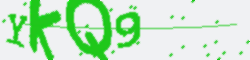
\includegraphics[width=1\linewidth]{imgs/textcaptcha/YKQ9.png}} 
        \\ а)
    \end{minipage}
    \begin{minipage}[h]{0.45\linewidth}
        \center{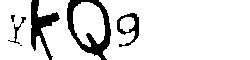
\includegraphics[width=1\linewidth]{imgs/textcaptcha/out.png}} 
        \\ б)
    \end{minipage}
    \caption{Изображения CAPTCHA: а) -- сгенерированное изображение, б) -- 
    результат обработки.}
    \label{fig:example-captcha}
\end{figure}

\vspace{-0.7cm}

\textbf{Подготовка датасета для CAPTCHA с изображениями}

Большинство предобученных моделей компьютерного зрения, таких как YOLOv8, обучены 
на датасете COCO~\cite{COCO}, содержащем изображения высокого качества с четкими 
контурами и однозначной аннотацией объектов. Однако CAPTCHA с изображениями имеют 
принципиально иные характеристики: они могут включать в себя размытие, наложенные 
артефакты, искажения, шумы, повторяющиеся элементы и искусственно пониженное 
разрешение. Все это снижает эффективность использования стандартных датасетов и 
моделей, не адаптированных под такие условия.

Для обеспечения высокой точности в задаче автоматического решения CAPTCHA 
необходимо подготовить собственный набор данных, приближенный к реальным условиям 
использования. Наиболее эффективным методом является автоматизированный парсинг 
изображений CAPTCHA, представленных на web-сайтах, использующих визуальные 
CAPTCHA-решения, такие как Google reCAPTCHA v2.

Использование реальных CAPTCHA, собранных в автоматическом режиме, имеет ряд 
преимуществ по сравнению с синтетической генерацией данных:
\begin{enumerate}
    \item изображения содержат разнообразные сцены, освещение, углы обзора и 
    уровни шума, что положительно влияет на способность модели к обобщению;
    \item присутствует большое количество уникальных объектов на фоне, в том 
    числе в частично перекрытых и смазанных вариантах;
    \item отсутствует необходимость в ручной генерации изображений и создании 
    дополнительных искажений для повышения реалистичности;
    \item возможно извлекать текстовые инструкции к CAPTCHA, что позволяет 
    соотносить каждое изображение с требуемым классом.
\end{enumerate}

Для парсинга CAPTCHA необходим автоматизированный сценарий взаимодействия с 
браузером с использованием библиотеки Selenium~\cite{Selenium}. Данный подход 
позволяет воспроизвести действия пользователя при работе с CAPTCHA, обходя при 
этом ручной ввод. Для обеспечения стабильной работы и масштабируемости процесса 
применяется браузерная автоматизация через WebDriver (в частности, ChromeDriver).

Функциональность парсера включает следующие ключевые этапы:
\begin{enumerate}
    \item поиск iframe-элемента, содержащего чекбокс <<Я не робот>>, и эмуляция 
    клика по нему для инициирования визуальной CAPTCHA;
    \item ожидание загрузки CAPTCHA и извлечение изображения с заданием (включая 
    его URL или пиксельный снимок);
    \item извлечение информации о структуре сетки (количество строк и столбцов), 
    на которую разбито изображение CAPTCHA;
    \item получение текста задания, содержащего имя объекта (например, <<выберите 
    все изображения с мотоциклами>>), для последующего использования в аннотации 
    данных.
\end{enumerate}

Типичная CAPTCHA представляет собой изображение, разделенное на сетку из 3×3 или 
4×4 ячеек, каждая из которых может содержать фрагмент сцены. При этом 
пользователю предлагается выбрать ячейки, в которых присутствует объект заданного 
класса. Процесс парсинга может быть представлена блок-схемой на рис.~
\ref{fig:captcha-flow}.

\begin{figure}[H]
    \centering
    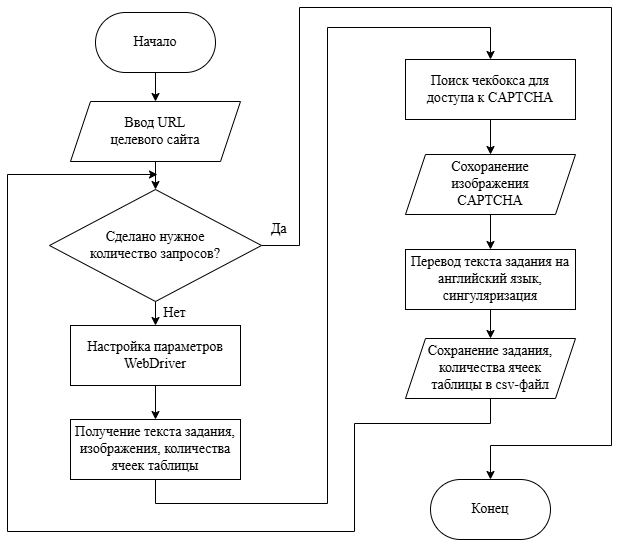
\includegraphics[width=0.6\textwidth]{
        imgs/imagecaptcha/image_captcha_flow.png
    }
    \caption{Блок-схема процесса парсинга CAPTCHA.}
    \label{fig:captcha-flow}
\end{figure}
\vspace{-0.5cm}

Полученные изображения и метаданные (включая текст задания и параметры сетки) 
используются для формирования обучающего датасета, пригодного для дообучения 
модели YOLOv8 в задачах классификации и сегментации объектов.

После получения достаточного количества изображений для составления датасета 
необходимо провести их предварительную обработку и разметку. Это один из 
самыхважных этапов работы, поскольку от качества разметки напрямую зависит 
точность и эффективность последующей работы модели.

Для создания меток используется инструмент CVAT (Computer Vision Annotation Tool) 
-- многофункциональное веб-приложение с поддержкой аннотации объектов с помощью 
полигонов, прямоугольников и других форм. CVAT позволяет экспортировать разметку 
напрямую в формат, совместимый с YOLO~\cite{CVAT}.

Поскольку CAPTCHA-изображения часто содержат объекты с нечеткими контурами, 
наложением и визуальными искажениями, особенно важно использовать ручную точную 
разметку, а не ограничиваться автоматическими методами. Выделение объектов должно 
проводиться как можно точнее, с учетом геометрии контуров. На рисунке ниже 
представлен пример изображения с размеченными объектами:

\begin{figure}[H]
    \centering
    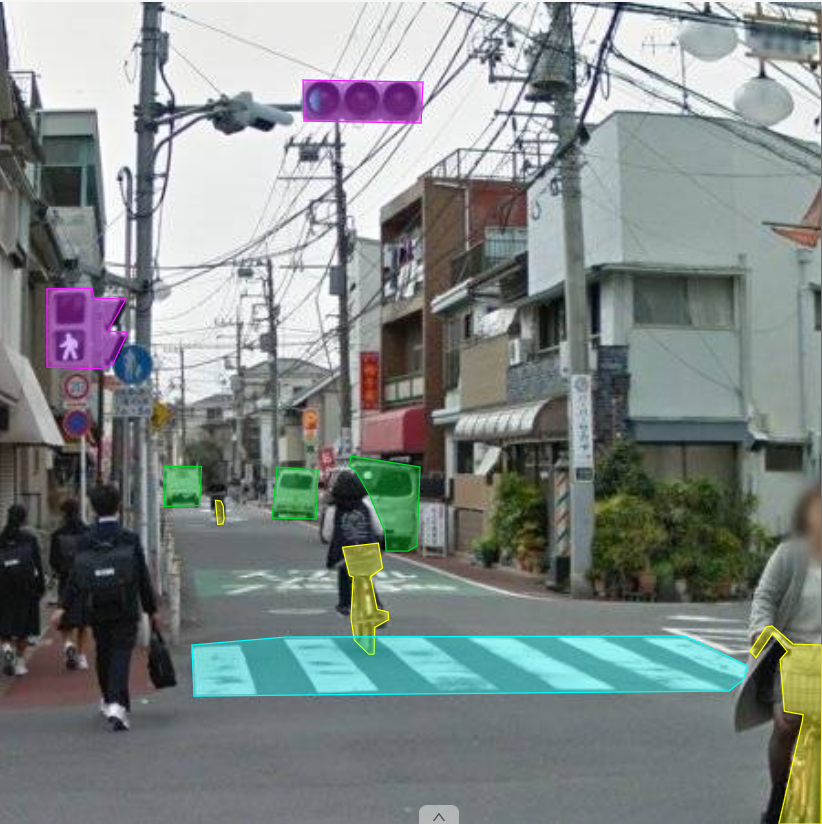
\includegraphics[width=0.9\linewidth]{imgs/imagecaptcha/captcha-poligons.png}
    \caption{Пример разметки изображения с тестовой CAPTCHA.}
    \label{fig:mask-captcha}
\end{figure}
\vspace{-0.5cm}

Кроме того, разметка позволяет учесть сразу несколько объектов разных классов на 
одном изображении, что особенно характерно для CAPTCHA, где в одной сетке могут 
одновременно находиться, например, автомобили и автобусы. Такой подход 
положительно влияет на обобщающую способность модели.

В случае, если количество данных по отдельным классам окажется недостаточным, 
можно дополнительно использовать методы аугментации: вращение, масштабирование, 
искажение цвета и контраста. Однако при хорошо организованном парсинге и разметке 
зачастую удается обойтись без аугментации.

Кроме того, для корректного обучения модели YOLO требуется создать иерархическую 
структуру папок, в которой изображения и соответствующие метки будут разделены на 
тренировочную и валидационную выборки. Стандартная структура включает следующие 
директории:
\begin{enumerate}
    \item директория train -- содержит тренировочную выборку:
    \begin{enumerate}
        \item директория images -- изображения;
        \item директория labels -- метки к изображениям.
    \end{enumerate}
    \item директория val -- содержит валидационную выборку:
    \begin{enumerate}
        \item директория images -- изображения;
        \item директория labels -- метки к изображениям.
    \end{enumerate}
\end{enumerate}

Набор классов, пути к выборкам и параметры конфигурации задаются в YAML-файле, 
который передается при обучении модели. Содержимое такого файла для данной 
модели:

\begin{code}
    \captionof{listing}{
        \label{code:train-captcha}Параметры конфигурации для обучения модели
    }
    \vspace{-0.75cm}
    {\small
        \inputminted[mathescape,linenos,frame=lines,breaklines]{yaml}{code/imagecaptcha/train_captcha.yaml}
    }
\end{code}
\vspace{-0.4cm}
